\documentclass{article}
\usepackage[utf8]{inputenc}
\usepackage{verbatim}
\usepackage{tikz}

\usetikzlibrary{shadings, patterns, shapes.geometric}

\title{CSE 300 Practice on tikZ}
\author{Your Roll}
\date{July 20, 2019}

\tikzstyle{myBox} = [rectangle, text centered, text width=3cm, draw=blue]

\begin{document}
\maketitle



\section{picture environment}

\setlength{\unitlength}{1cm}

\begin{verbatim}
\begin{picture}(width, height)
     \put(starting point){object}
\end{picture}
\end{verbatim}

\subsection{Different Objects}

\begin{description}
    \item[Line] \verb|\put(starting point){\line(direction){length}}|\\
    Such as; \verb|\put(0,0){\line(0,1){2}}|
    \item[Vector] \verb|\put(starting point){\vector(direction){length}}|\\
    Such as; \verb|\put(2,1){\vector(1,0){2}}|
    \item[Circle] \verb|\put(center){\circle{radius}}|\\
    Such as; \verb|\put(5,1){\circle{1.2}}|
    \item[Filled Circle] \verb|\put(center){\circle*{radius}}|\\
    Such as; \verb|\put(9,1){\circle*{1}}|
\end{description}

\begin{picture}(2,2)
\put(0,0){\line(0,1){2}}
\put(2,1){\vector(1,0){2}}
\put(5,1){\circle{1.2}}
\put(9,1){\circle*{1}}
\end{picture}

\section{tikz package}

There are mainly two ways for using tikz package

\begin{itemize}
    \item
    \begin{verbatim}
        \begin{tikzpicture}[options]
            <tikz code>
        \end{tikzpicture}
    \end{verbatim}
    \item \verb|\tikz[options]{tikz codes}|
\end{itemize}

\subsection{tikz codes}
\verb|\path[option1][option2] <specification>;|\\
This is the most basic command inside tikzpicture environment. We will first learn about the usage of option1.

\subsubsection{Option1}
draw, fill, pattern, clip, shade, use as bounding box.\\
\quad Example1: \verb|\path[draw], \path[fill], & so on|\\
\quad Example2: \verb|\path[draw, fill], \path[draw, clip], & so on|\\

\textbf{Note:} \verb|\path| with these options can be combined to \verb|option1|,\\

\qquad \verb|\path[option1]|$\equiv$\verb|\option1|\\

Example: \verb|\draw, \fill, \drawclip, etc.|

\subsubsection*{Using \textbackslash draw}

\quad~
\begin{tikzpicture}
    \draw (1,0) -- (0,0) -- (0,1);
\end{tikzpicture}

\verb|\draw (1,0) -- (0,0) -- (0,1);|

\vskip25pt
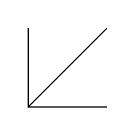
\begin{tikzpicture}
    \draw (1,0) -- (0,0) -- (0,1) (0,0) -- (1,1);
\end{tikzpicture}

\verb|\draw (1,0) -- (0,0) -- (0,1) (0,0) -- (1,1);|

\vskip25pt
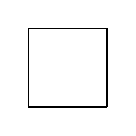
\begin{tikzpicture}
    \draw (1,0) -- (0,0) -- (0,1) -- (1,1) -- (1,0);
\end{tikzpicture}

\verb|\draw (1,0) -- (0,0) -- (0,1) -- (1,1) -- (1,0);|

\vskip25pt
\begin{tikzpicture}
    \draw (0,0) rectangle (1,2);
    \draw (3,0)--(4,0)--(4,2)--cycle;
\end{tikzpicture}

\verb|\draw (0,0) rectangle (1,2);|\\
\quad\verb|\draw (3,0)--(4,0)--(4,2)--cycle;|

\vskip25pt
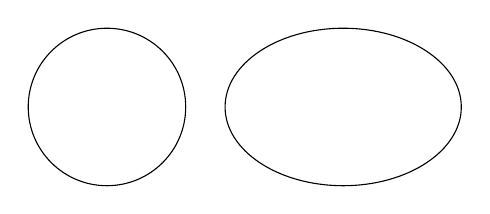
\begin{tikzpicture}
    \draw (0,0) circle[radius=1cm];
    \draw (3,0) circle[x radius = 1.5cm, y radius=1cm];
\end{tikzpicture}

\verb|\draw (0,0) circle[radius=1cm];|\\
\quad\verb|\draw (3,0) circle[x radius = 1.5cm, y radius=1cm];|

\vskip25pt
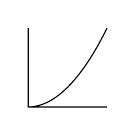
\begin{tikzpicture}
    \draw (1,0)--(0,0)--(0,1) (0,0) parabola (1,1);
\end{tikzpicture}

\verb|\draw (1,0)--(0,0)--(0,1) (0,0) parabola (1,1);|

\vskip25pt
\begin{tikzpicture}
    \draw (1,0) .. controls (2,2) .. (3,0);
\end{tikzpicture}

For drawing a curved line along with the start and end co-ordinate, you must provide the control point.\\
\verb|\draw (1,0) .. controls (2,2) .. (3,0);|

\vskip25pt
\begin{tikzpicture}
    \draw (0,0) arc[start angle=30, end angle=90, radius=1cm];
    \draw (3,0) arc(30:90:3cm);
\end{tikzpicture}

We can also draw arcs.\\
\verb|\draw (0,0) arc[start angle=30, end angle=90, radius=1cm];|\\
\verb|\draw (3,0) arc(30:90:3cm);|


\vskip25pt
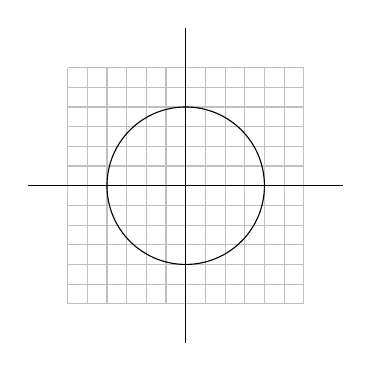
\begin{tikzpicture}
    \draw (-2,0) -- (2,0);
    \draw (0,-2) -- (0,2);
    \draw (0,0) circle [radius=1cm];
    \draw[step=0.25cm, opacity=0.25] (-1.5,-1.5) grid (1.5,1.5);
\end{tikzpicture}
We need to use the grid command for drawing grids. We can add some additional features for grid in option2\\
\verb|\draw[step=0.25cm, opacity=0.25] (-1.5,-1.5) grid (1.5,1.5);|\\
By default step is set at 1cm \& opacity at 1.

There are numerous options available under option2. Everything under option2 can also be used as option for the environment as a whole.\\
Everything drawn under the following environment will be red:\\
\begin{verbatim}
    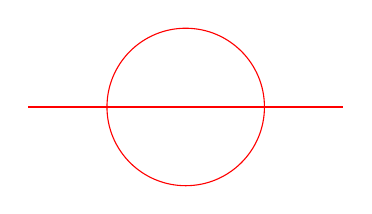
\begin{tikzpicture}[color=red]
        \draw (-2,0)--(2,0);
        \draw (0,0) circle[radius=1cm];
    \end{tikzpicture}
\end{verbatim}

Some example options:\\
\begin{itemize}
    \item line width=dim, ultra thin, very thin, thin(default), semithick, thick, very thick, ultra thick
    \item dash pattern=on dim. off dim. \ldots, solid, dotted, densely dotted, loosely dotted, dash dot, dash dot dot, double, double=color name, double distance=dim
    \item line cap= $<$ rect, round, butt $>$, arrows= $<$ start arrow kind - end arrow kind $>$
\end{itemize}

\vskip25pt
\begin{tikzpicture}[transform canvas={xshift=3cm, yshift=-5cm}, scale=1.5]
    \draw[color=red, rotate=30, line width=1pt, double, double distance=5mm, double=pink] (-2,0) -- (2,0);
    \draw[color=blue, line width=1pt, dash pattern=on 2pt off 3pt on 4pt off 4pt] (0,0) circle [radius=1cm];
\end{tikzpicture}

\vskip25pt
\begin{tikzpicture}
    \draw[arrows= <->] (-3,0)--(3,0);
\end{tikzpicture}
\newpage
\subsubsection*{Using other commands}
\textbf{Using \textbackslash fill}\\

\begin{tikzpicture}
    \fill[color=yellow] (0,0) rectangle (3,4);
    \draw[color=red] (0,0) rectangle (3,4);
\end{tikzpicture}

\verb|\fill[color=yellow] (0,0) rectangle (3,4);|\\
\verb|\draw[color=red] (0,0) rectangle (3,4);|

\vskip1cm

\textbf{Using \textbackslash shading}\\

\begin{tikzpicture}
    \shade[shading=radial] (0,0) rectangle (3,4);
\end{tikzpicture}

\verb|\shade[shading=radial] (0,0) rectangle (3,4);|\\

Different kinds of shading are there: axis, radial, ball\\

Besides, shading angle can be defined as \verb|shading angle=angle value|\\

Shading color can be defined too:\\
left color= value, right color = value\\
top color=value, bottom color=value, middle color=value\\
inner color=value, outer color=value\\

For additional shading options use tikzlibrary shadings by writing the following command in your preamble: \verb|\usetikzlibrary{shadings}|\\
Different options available under the shadings library are shading=color wheel, upper right=color name, etc.\\

\textbf{Using \textbackslash pattern}\\
For patterns, we have to use another tikzlibrary called patterns. Some examples are as follows:
\vskip1cm
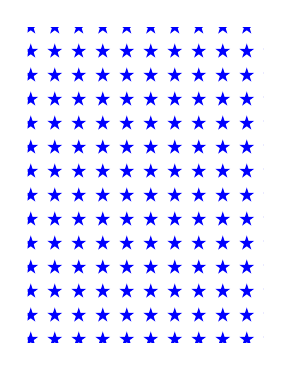
\begin{tikzpicture}
    \pattern[pattern=fivepointed stars, pattern color=blue] (0,0) rectangle (3,4);
\end{tikzpicture}\\

There are so many patterns. Some are: dots, fivepointed stars, vertical lines, grid horizontal lines, bricks, checkboard, checkboard light gray, etc.\\

We can also set pattern color=value.\\
\begin{verbatim}
  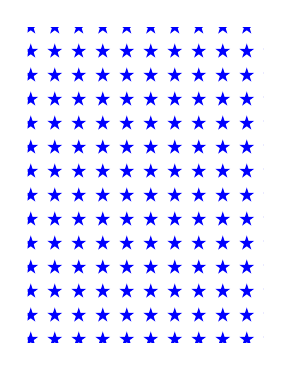
\begin{tikzpicture}
    \pattern[pattern=fivepointed stars, pattern color=blue] (0,0) rectangle (3,4);
  \end{tikzpicture}
\end{verbatim}

\subsubsection*{Working with \textbackslash node}
\verb|\node[options](label){<text>};|\\
\verb|\node[options](label) at (coordinate){<text>};|\\

\begin{tikzpicture}
    \draw[<->,thick] (3,0)--(0,0)--(0,3);
    \fill (1.5,1.5) circle[radius=2pt];
    \node[below] at (3,0){$x$};
    \node[left] at (0,3){$y$};
    \node[left] at (0,0){O};
    \node[above](n1) at (1.5,1.5){A};
    \node[left] at (n1){B};
\end{tikzpicture}

For getting the above figure the required code is as follows:\\

\begin{verbatim}
\begin{tikzpicture}
    \draw[<->,thick] (3,0)--(0,0)--(0,3);
    \fill (1.5,1.5) circle[radius=2pt];
    \node[below] at (3,0){$x$};
    \node[left] at (0,3){$y$};
    \node[left] at (0,0){O};
    \node[above](n1) at (1.5,1.5){A};
    \node[left] at (n1){B};
\end{tikzpicture}
\end{verbatim}

\subsection{Flow Chart}

At first we will learn how to connect two points with two labelled nodes.

\begin{tikzpicture}
    \node[left](n1) at (2,0){A};
    \node[right] (n2) at (5,3){B};
    \draw (n1) -| (n2);
\end{tikzpicture}

The corresponding code:\\
\begin{verbatim}
\begin{tikzpicture}
    \node[left](n1) at (2,0){A};
    \node[right] (n2) at (5,3){B};
    \draw (n1) -| (n2);
\end{tikzpicture}    
\end{verbatim}


For generating different geometric shapes, we have to use tikzlibrary called `shapes'. [\verb|\usetikzlibrary{shapes.geometric}|]\\

Different shapes under the library are: diamond, ellipse, trapezium, semicircle, cylinder, regular polygon, kite, etc.


\begin{tikzpicture}
    \node[draw, diamond]{decision?};
\end{tikzpicture}

\verb|\node[draw, diamond]{decision?};|\\

\subsubsection*{Example}

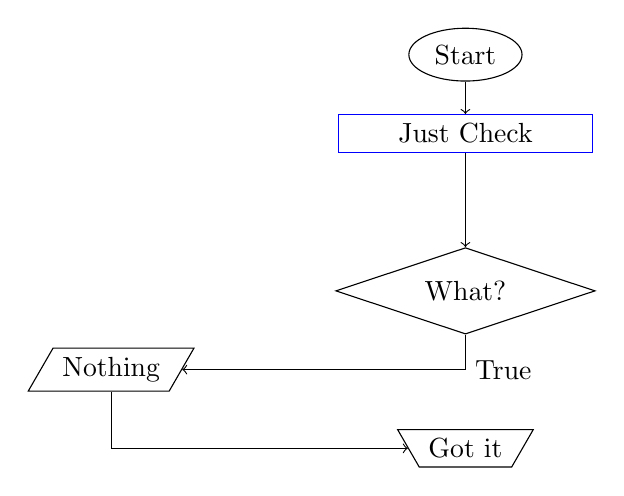
\begin{tikzpicture}
    \node[draw, ellipse] (start){Start};
    \node[myBox, below of=start] (mB){Just Check};
    \node[draw, diamond, align=center, text width=2cm, aspect=3, yshift=-1cm, below of=mB, inner sep=2pt] (decision){What?};
    \node[draw, trapezium, trapezium left angle=60, trapezium right angle=120, left of=decision, yshift=-1cm, xshift=-3.5cm] (l1){Nothing};
    \node[draw, trapezium, trapezium left angle=120, trapezium right angle=120, below of=decision, yshift=-1cm] (l2){Got it};
    
    \draw[->] (start)--(mB);
    \draw[->] (mB)--(decision);
    \draw[->] (decision.south) |- node[right]{True} (l1.east);
    %\draw[->] (decision.west) node[below]{True} -| (l1.north);
    \draw[->] (l1.south) |- (l2.west);
\end{tikzpicture}\\

\begin{itemize}
    \item Ellipse: \verb|\node[draw, ellipse] (label){text};|
    \item Diamond: 
    \begin{verbatim}
        \node[draw, diamond, align=center|left|right, text width=dim,
        
        aspect=x:y, xshift=dim, yshift=dim, <below of|left of|right of>=node,
        
        inner sep=dim] (label){text};
    \end{verbatim}
    \item Trapezium:
    \begin{verbatim}
        \node[draw, trapezium, trapezium left angle=val,
        
        trapezium right angle=val, xshift=dim, yshift=dim,
        
        <below of|left of|right of>=node,] (label){text};
    \end{verbatim}
\end{itemize}

You can write your own object using the command \verb|\tikzstyle{objectName}=[options]|. For example the rectangular box above within blue bounding box is drawn as custom object:

\begin{verbatim}
    \tikzstyle{myBox} = [rectangle, text centered, text width=3cm, draw=blue]
\end{verbatim}

The command used to draw the aforementioned object:

\begin{verbatim}
    \node[myBox, below of=start] (mB){Just Check};
\end{verbatim}

Now,  let's focus on connecting the shapes: We already know how to draw a line with directional arrowheads between two nodes. We use the same command here:

\verb|\draw[->] (start)--(mB);|\\
Here, the tricky part is if we want to draw connection from any definite side, we have to mention (east$\|$west$\|$north$\|$south) side of the particular object/node. Such as,\\
\begin{verbatim}
    \draw[->] (l1.south) |- (l2.west);
\end{verbatim}\\

If we want to add tag to any connection, we use the following code:
\begin{verbatim}
    \draw[->] (decision.south) |- node[right|left|above|below]
    {tag} (l1.east);
\end{verbatim}

\end{document}
